%% ID: Eliza_washing_line
%% TITLE: Towel on a Washing Line
%% TYPE: question
%% QUESTIONTYPE:  numerical
%% CONCEPTS: forces, vectors2, newtoni
%% VIDEOS: 
%% LEVEL: 2
%% TOPIC: mechanics/statics
%% ORDER: 10

\begin{problem}[Eliza_washing_line] 
{\exposition{Consider a wet towel of mass $2m$ as in Figure \ref{fig:Statics_washing_line_unmarked}. It is hung on a length $4a$ of light inextensible string by two pegs a distance $a$ from each end. The ends of the string are attached to two washing poles $4b$ apart, where $b < a$.} \question{Give expressions for the tensions in all three parts of the string in terms of $m$, $g$, $a$ and $b$.}
\exposition{
\begin{figure} [h]
	\centering
	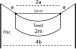
\includegraphics[width=0.4\textwidth]{Statics_washing_line_unmarked}
	\caption{}
	\label{fig:Statics_washing_line_unmarked}
\end{figure}}
\hinta{Define an angle in terms of the lengths $a$ and $b$, then try resolving forces about one of the pegs.}}
{\textit{Created for the Rutherford School Physics Project by EM and PS.}}
{\begin{figure} [h]
	\centering
	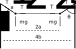
\includegraphics[width=0.4\textwidth]{Statics_washing_line}
	\caption{}
	\label{fig:Statics_washing_line}
\end{figure}
This question models the washing as two individual masses, each of mass $m$, hanging on the line as in Figure \ref{fig:Statics_washing_line}. By symmetry, $T\s{1} = T\s{3}$. We can resolve vertically about one of the pegs to obtain the equation:
\begin{equation*}	T\s{1}\cos{\theta} = mg	\end{equation*}
\begin{figure} [h]
	\centering
	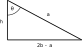
\includegraphics[width=0.4\textwidth]{Statics_washing_triangle}
	\caption{}
	\label{fig:Statics_washing_triangle}
\end{figure}
We can define $\theta$ in terms of the triangle shown in Figure \ref{fig:Statics_washing_triangle}, where $2b - a$ is the horizontal distance between the peg and the washing pole. Using Pythagoras:
\begin{equation*}	h = \sqrt{a^{2} - \left(2b - a\right)^{2}} = \sqrt{a^{2} - 4b^{2} + 4ab - a^{2}}	\end{equation*}
\begin{equation*}	h = 2\sqrt{b\left(a - b\right)}	\end{equation*}
Therefore $\cos{\theta} = \frac{2\sqrt{b\left(a - b\right)}}{a}$. This gives us our expression for $T\s{1}$:
\begin{equation*}	T\s{1} = \frac{mg}{\cos{\theta}}	\end{equation*}
\begin{equation*} 	T\s{1} = \frac{mga}{2\sqrt{b\left(a - b\right)}}	\end{equation*}
To obtain an expression for $T\s{2}$ we must first resolve horizontally about one of the pegs:
\begin{equation*}	T\s{2} = T\s{1}\sin{\theta}	\end{equation*}
\begin{equation*}	T\s{2} = \frac{mg}{\cos{\theta}}\sin{\theta} = mg\tan{\theta}	\end{equation*}
Returning to our triangle we find that $\tan{\theta} = \frac{a\left(2b - a\right)}{2\sqrt{b\left(a - b\right)}}$. This gives us our final result:
\begin{equation*}	T\s{2} = \frac{mga\left(2b - a\right)}{2\sqrt{b\left(a - b\right)}}	\end{equation*}

\answer{The tensions in the parts of the string are $T\s{1} = T\s{3} = \frac{mga}{2\sqrt{b\left(a - b\right)}}$ and T\s{2} = \frac{mga\left(2b - a\right)}{2\sqrt{b\left(a - b\right)}}}

}
\end{hint}